\documentclass[a4paper]{article}

\usepackage[utf8]{inputenc}

\usepackage{url}
\usepackage[hidelinks]{hyperref}

\usepackage{caption}

\usepackage{listings}

\usepackage{color}

% *** GRAPHICS RELATED PACKAGES ***
%\usepackage[pdftex]{graphicx}
\usepackage{graphicx}
%\usepackage[dvips]{graphicx}
% to place figures on a fixed position
\usepackage{float}

\usepackage[margin=1in]{geometry}

\title{P2P – syllabus}
\author{}
\date{}


\begin{document}

\maketitle

\tableofcontents

\section{Introduction}

Compared to traditional client-server connections peer-to-peer solutions (P2P) offer more direct and dynamic
alternatives. They provide searching services in a global network and allow direct, point to point data transfers
bypassing the administrative and performance bottlenecks of servers.
The well-know and most used P2P applications -- like file exchange, VoIP and on-line gaming -- affects many users and
generate the significant portion of today's Internet traffic. Covering all aspects of P2P network during this lab would
be impossible therefore only some key parts will be demonstrated. Since file transfer is currently to most utilized
application we are going to cover that during this lab.

\section{P2P file exchange}

The first system specifically designed for file exchange called \emph{Napster} was released in 1999. The file exchange
networks were growing rapidly after that, several architectures had been developed and had been categorized  into 3
main categories. This chapter gives an overview on each and then discusses BitTorrent in detail which is going to be
the main focus during this lab.

\subsubsection{Client-server systems}

The architecture of Napster is considerably simple. The basis of it is one central server and each user is connected to
this server with its client program. Downloading is controlled by the central server however the data transfer is
between the two requesting and the offering clients directly without going through the server. This property makes it
eligible Napster to be categorized as a P2P network due to utilizing the storage capacity and network access bandwidth
of all of its clients. An obvious shortcoming of Napster's architecture is the reference to the central server park --
shutdown of that would bring down the whole network. This had happened several times in the past due to ongoing legal
procedures between RIAA (American copyright protection entity) and Napster because of the contents that were available
on the network.

The focus transitioned on changing the principal design of the architecture and was looking for a solution that doesn't
rely on central entities i.e. it's fully distributed. Others were just trying to address security related problems. The
resulting architecture had the clients connect to a server but the server itself did not store an information about the
clients and many smaller servers were in operation instead of just one central entity. The most notable implementation
of this architecture is DirectConnect.

\subsubsection{Distributed systems}

After the fall of Napster it had been realized that the main vulnerability of these systems is the presence of the
central server. Later on as a result of repeated strikes against DirectConnect based networks most of the file exchange
users started looking for a system which operates in a fully distributed way i.e. it doesn't have any central entity.
The distributed architecture had its own cons compared to the client-server based approach. In distributed systems the
number of network hops could be arbitrarily large resulting in greater network traffic in the network itself and in
increased execution time of downloads, queries, etc. Another theoretical problem is that connecting to a distributed
network is not trivial -- due the missing central server -- the client who wants to connect has to obtain the network
address of some already connected client. Furthermore network administration had become virtually unmanageable.

Around the year 2000 several networks had been operated based on the principles described above. Almost every
programmer was developing P2P file exchange software in his free time. A variety of different but short-lived solutions
had been introduced in this era. However some of the systems have survived and gain popularity for example Gnutella
which is still one of the most popular network in some countries.

Gnutella newtork is truly peer-to-peer which means that its only contains clients communicating with each other; it
doesn't utilize any central or globally reachable component. As mentioned before there is a problem arising from new
client connections: it's necessary to know at least one already connected client. Initially there was no well
established methodology for that resulting in spreading the word about some clients that were already connected between
people to be able to connect to the network. There had been some search algorithms introduced to overcome this however
these did not operate effectively in global scale.

After a client got hold of a Gnutella member it could initiate a connection to it with a greeting message. The peer
receiving this message replies and indicates its availability. Furthermore it forwards the message to all of its known
peers - naturally these messages utilized a Time-To-Live (TTL) mechanism. This process repeats until the TTL reaches 0.
During the message's lifetime it gets process by a lot of network members -- technically all peers in 6 hops distance
from the edge peer. Afterwards the connecting peer initiates a connection to all reachable peers as a result then it is
tightly coupled to the network.

Gnutella provides almost complete security against legal concerns because the complete network is technically
non-discoverable. This non-discoverable property is one of the greatest drawbacks of it because due to the client's
relatively small horizon it it impossible to know many peers are using the network without being able to monitor the
whole Internet. Still there are only approximations about the total number of users which says it's around the
magnitude of 1000 connection per 1 peer.

The search messages are processed similarly to the connection initiation messages. The client floods the search message
to all of its connected peers. Those process the query and if any has a positive match it sends back a reply. The
message is then flooded onwards -- TTL mechanism still applies. In this way the search request	traverses all the way
through the client's horizon and the originating peer receives all the positive matches. The reply messages may contain
new peers that can be used for establishing new connections if the originating peer would like to broaden its horizon.

\subsubsection{Hierarchical systems}

The hierarchical systems combine the advantages of the previously described client-server and pure P2P networks.
It doesn't have central entities with global availability however not all peers are equal: some of the entities has
special responsibilities.
This type of network can be imagined as the special purpose entities -- a.k.a. super-clients -- are connected to each
other in a P2P fashion while regular clients are connected to these super-clients in a client-server fashion.
Kazaa (FastTrack) operates based on this principle.

Fastrack is basically based on later versions of Gnutella where only the \emph{Ultrapeers} are eligible to be connected
to the Gnutella network itself while the leaf clients can only connect to Ultrapeers. The Ultrapeers responsiblity
beside processing their own search operations is to serve the connected regular clients and take over their traditional
P2P tasks. In the Kazaa network the Ultrapeers are called \emph{Superpeers}.

When the user starts the client program that uses a proprietary algorithm to decide the role in which it will operate.
If it is going to be a Supernode it is trying to establish connections with other Supernodes. Due to the encrypted
communication it is unknown how Supernodes find each other but it's known that the client software contains a
hard-coded list of Supernodes that gets updated with each release. The Supernode under connection tries to connect to
Supernodes chosen from this list until it successfully connects to one of them. After successful connection the other
Supernodes will send the current list of Supernodes in the network so the newly connected Supernode can update its
database. It is unknown that how the list of Supernodes is created but it's likely that it is similar to the process
used by Gnutella. The protocol used between Supernodes are not known in details due the encrypted nature of the
communication but measurements showed that a Supernode connects to 25 other Supernodes on average.

FastTrack architecture is a fine fusion between the client-server and the pure P2P networks. The Supernodes backbone
that replaces the central server entity provides a scalability and high-availability. Flooding only takes part between
Supernodes as a consequence as more ordinal peers connect to the network the network traffic is not growing
proportionally -- it only increases between the high bandwidth Supernodes. This architecture resembles the architecture
of Skype -- not accidentally as the same developer team was responsible for developing both systems.

\section{BitTorrent}
A 2001-ben született BitTorrent eredeti célja a szerverek terhelésmentesítése volt. A probléma adott: van egy szerver,
amiről túl sokan akarják ugyanazt az állományt egyszerre letölteni. A szerver ilyenkor lelassul, rosszabb esetben
összeomlik. Az ötlet egyszerű: miért mindenki a szerverről tölti le az adatokat, mikor azok egy része a többi
letöltőnek is megvan már? A megoldás tehát az, hogy az állományokat kis részegységekre osztjuk, és ezeket mindenki
tetszőleges sorrendben letöltheti, nem csak a központi gépről, hanem a többi letöltőtől is, akinek megvan az adott
darab. Így minél többen töltenek le egy darabot egymástól, annál inkább elterjed a letöltők között, mind jobban
tehermentesítve a szervert. A megvalósításhoz két különböző funkciójú központi elemre is szükség van. A Seeder maga a
szerver, mely eredetileg, teljes egészében hozzáférést biztosít az eredeti állományhoz. A Tracker pedig egy olyan
szerver, mely nyilvántartja a letöltések menetét, így az újonnan csatlakozó kliensek számára meg tudja mondani, hogy az
állomány egyes darabjai mely klienseken érhetőek el.

Hálózatméret szempontjából ez a koncepció tulajdonképpen a Napster és DirectConnect között végbemenő átmenet
folytatása. Míg a Napsternél egy globálisan egységes hálózat megalkotása volt a cél, addig a DirectConnectnél már
inkább kisebb, tematikus hálózatok létrejöttét tűzték ki célul. Az ilyen kisebb hálózatokhoz ugyanis csak azok
csatlakoztak, akik érdekeltek voltak az adott közösség által megosztott állományokban, így egy-egy hálózatban kevesebb
"felesleges" állomány volt megosztva. A BitTorrent ezt a gondolatot viszi el a végsőkig: itt egyenesen olyan
mikro-hálózatok alakulnak ki, amelyek csak egyetlen egy állomány megosztásáért felelősek. Persze ha valaki akar,
egyszerre több ilyen hálózatnak is tagja lehet, ám számára így is csak a hasznos állományok megosztását segítő
hálózatoknak kell tagja lennie. Ezeket a gondolatokat igazolják azok a mérések is, melyek szerint egy adott
állománymegosztó rendszerben a forgalom mintegy 90%-át a megosztott állományok csupán 5-10%-a adja.

E tulajdonság miatt a rendszer rendkívül gyors letöltést biztosít, sokszor a letöltési sávszélesség jelenti a szűk
keresztmetszetet. Ezért, bár a rendszer jelentősen eltér a többi állománymegosztó rendszertől, mégis hamar felismerték
a benne rejlő lehetőséget. Kisebb módosításokra szükség volt ugyan, ám – köszönhetően a nyílt forráskódnak – egyre
újabb verziók jelentek meg, melyek mind alkalmasabbá váltak az állománymegosztásra; pontosabban a letöltésre, hiszen a
program ezen kívül semmilyen más funkcióval nem rendelkezett.

Az állománymegosztáshoz a gyakorlatban – az eredeti elgondoláshoz képest – a következő módosításokat hajtották végre:
vannak speciális weboldalak, ahonnan letölthetőek az úgynevezett torrent állományok. Ezek az oldalak sokfélék lehetnek,
és ugyanazt a torrent állományt több ilyen oldalon is megtalálhatjuk. Ezek alapján a torrent állományok alapján pedig
megtalálhatjuk a számunkra megfelelő Tracker és Seeder szervereket.

További különbség, az eredeti elképzeléshez képest, hogy a Seeder szervere elvesztette kiemelt szerepét. Az új
elgondolás szerint amint valaki befejezte a letöltést, azaz az állomány összes részével rendelkezik, maga is Seederré
válik. Így idővel a Seederek száma is megnő a hálózatban, még jobban gyorsítva a letöltést. Ennek ellenére a
terminológia továbbra is Seedernek nevezi azokat a klienseket, amelyek az egész állományt megosztják a többi kliens
számára (így azt is, aki először tette közzé az állományt).

A csatlakozáshoz, illetve a letöltés megkezdéséhez a felhasználóknak először egy torrent állományt kell letölteniük,
hogy ennek segítségével megtalálhatják a keresett állomány Trackerét és Seederét. A Tracker szerver segítségével ezután
megtalálhatják azokat a klienseket is, amelyek éppen az állomány különböző darabjait töltötték le, így jelenleg róluk
is elérhető. Az újabb verziókban a torrent állományok már több Trackerre és Seederre is hivatkoznak, így egyik leállása
esetén a letöltések zavartalanul folyhatnak tovább.

Az állományok megosztása természetesen itt máshogy történik, mint a többi állománycserélő rendszer esetében. A
BitTorrentet egyes állományok megosztására, letöltésére találták ki, nem pedig az osszunk meg minél több állományt elv
kielégítésére. Így ez nem támogat olyan lehetőségeket, mint teljes könyvtárak megosztása.

A megosztáshoz először is választanunk kell egy Tracker szervert, vagy akár többet is. Ezután el kell készítenünk a
torrent állományunkat, amely ránk hivatkozik Seederként, a Tracker szerverekre pedig, mint Trackerek. Továbbá a
megosztani kívánt állományt fel kell darabolni, illetve minden egyes részének a hash értékét kiszámolni, és beleírni a
torrent állományba. Végül a torrent állományt publikálnunk kell valahol, hogy azt az érdeklődők megszerezhessék. Erre
szakosodott web-szerverek léteznek, amelyek különböző meta-információk megadása esetén keresési lehetőséget is
nyújtanak az elérhető torrent állományok által nyújtott állományokról.

Amikor a letöltők megszereztek egy-egy részt, akkor ezután azok is megosztják azt a többiek számára, úgy, hogy a
Tracker szervernek jelzik, hogy ez most már náluk is elérhető. Amikor egy letöltő a teljes állományt letöltötte, ő is
Seederré válik, így onnan kezdve a torrent állomány akár őt is megjelölheti forrásként.

A kliensprogramok bár nyílt forráskódúak, a freeriding megakadályozása érdekében általában implementálják azt az elvet,
hogy a letöltés sebessége legyen viszonylag arányos a feltöltési sebességével. Így megoldható, hogy senki se tudjon
"élősködni" a többi felhasználón.

Mivel a BitTorrent esetében olyan mikro-hálózatokról beszélhetünk, amelyek egy-egy állomány szétszórására jöttek létre,
nyílván nincs lehetőségünk keresések lefolytatására. Az egyes állományok keresésére általában a torrent állományok
tárolására szakosodott szerverek adnak lehetőséget. Ezeken a szervereken egy torrent állomány mellé elmenthetjük az
általa megosztott állomány meta-információit, így a web felületen lehetőségünk lesz arra, hogy ezek között keressünk.
Így tulajdonképpen az állomány keresése után egy torrent állományt kapunk, amely elvezet minket az adott állomány
mikro-hálózatához.

A torrent állomány segítségével felvehetjük a kapcsolatot egy Tracker szerverrel, ami ezután átirányít minket azokhoz a
kliensekhez, illetve a Seederhez, ahonnan az állomány egyes részeit letölthetjük. Miután egy-egy rész lejött, ezt a
Tracker megjegyzi, így az újabb klienseket már hozzánk is irányíthat.

Valójában az állomány egyes részei is alrészekre vannak osztva, így még a nagyon rövid tartamú letöltések esetén is
sikeres lehet a teljes állomány megszerzése. Amikor egy állomány részének alrészét letöltöttük valahonnan, a
kliensprogram előnyben részesíti ugyanazon rész más alrészeit. Így nagyobb eséllyel lesz meg nálunk egy teljes rész,
ami ezután már tőlünk is hozzáférhetővé válik. Természetesen ezelőtt a hash érték ellenőrzése is megtörténik, amellyel
biztosíthatjuk, hogy a rész hibamentesen letöltésre került. További optimalizálást jelent, hogy a Tracker számon
tartja, melyek azok a részek, amelyekkel a legkevesebb letöltő rendelkezik. Így egy új letöltőt arra utasít, hogy
először ezeket töltse le. Így egyrészt tehermentesítik a szervert, másrészt pedig biztosítják, hogy a hálózatban minden
egyes rész megfelelő számban rendelkezésre álljon, így ha a Seeder közben el is veszik a hálózatból, a ritkább részek
is elérhetőek maradnak. Ugyanakkor a klienseknek is előnyös a ritka részek letöltése. Hiszen ha egy-egy ilyen ritka
rész birtokába jut, nagyobb eséllyel fogják azt tőle letölteni, mint egy olyat, amely minden letöltőnél elérhető. Ezzel
garantálható, hogy többen töltenek le, vagyis növeli a globális letöltési sebességét, ezáltal biztosíthatja maga
számára a nagy letöltési sebességet is. Az állományok letöltése tehát úgy történik, hogy a lehető legtöbb olyan
klienshez csatlakozunk, melyeknek az állomány különböző részei már rendelkezésére állnak. Amikor egy-egy részt
letöltöttünk, azt mi is megosztjuk a közösséggel, így azok már tőlünk is elérhetővé válnak.

A letöltés ideje nyilván nagyon változó, szinte megjósolhatatlan. Az egész rendszerre jellemző a lassú indulás, majd a
fokozott növekedés. Eleinte ugyanis csak a Seederen találhatóak meg az állomány részei, így minden kliens onnan kezdi
letölteni azokat. Ezután azonban mind egyre több peeren lesz elérhető, vagyis azok fokozatosan leveszik a terhet a
Seederről, ezzel a rendelkezésre álló részek sávszélessége is tulajdonképpen egyre jobban nő a hálózat egészében.

A torrent állományokban a bencode módszert alkalmazzák az adatok kódolására. Ez egy string alapú kód, ami igen könnyen
visszafejthető. Ez a "nyelv" kétféle egyszerű és kétféle összetett típust használ. Az egyszerű típusok stringeket és
egész értékeket tárolnak, az összetett típusok pedig listákat és úgynevezett szótárakat, amikben egyes értékekhez más
értékeket rendelhetünk. Az összetett elemek természetesen más összetett elemeket is tárolhatnak.

Az integereket "i" kezdő és "e" befejező-karakterek közé kell írni, például a 13-at i13e-ként ábrázoljuk.

A stringek kódolása úgy történik, hogy a string hosszát decimális számként leírjuk, majd kettőspont után maga a string
következik. Például az "alma" string bencode megfelelője a 4:alma. Ebben az esetben tehát nem használunk
záró-karaktert, hanem a string hosszából tudjuk megállapítani hol fejeződik be.

A listák tetszőlegesen sok bencode eljárással ábrázolt adatot tartalmazhatnak, melyet az "l" és "e" karakterek közé
kell helyeznünk. Például az "l4:almai13ee" egy olyan kételemű listát ábrázol, melyben az első elem az "alma” string, a
második pedig a 13-as egész szám.

A szótárakat a listákhoz hasonlóan "d" és "e" karakterek között ábrázoljuk bencode kódolt karakterekkel, azonban itt
kettesével kell felsorolnunk az elemeket, melyekből az első a kulcs, a második pedig a hozzá rendelt érték lesz.
Például a "d4:almai13e5:körte5:nincse" egy olyan szótárat ír le, melyben az "alma" stringhez 13-at, a "körte"-hez pedig
"nincs"-et rendelünk.

\section{Topology-aware BitTorrent clients}

A peer-to-peer alkalmazások terjedésével, és a ma ugyan már csökkenő, de még mindig jelentős szerepükkel, nagy részt
hasítanak ki az Internet teljes forgalmából: egyes becslések szerint a peer-to-peer alkalmazások a teljes forgalomnak
akár 70\%-át is generálhatták egy időben. A gondot az okozza, hogy az overlay koncepció figyelmen kívül hagyj a
hálózati topológiát. A jelenleg legnépszerűbb BitTorrent alkalmazás nagyban növeli az ISP-k internetes linkekre
fizetett költségét az ISP-közi megnövekedett forgalom miatt. Ez az ISP-ket arra kényszeríti, hogy a felhasználók
peer-to-peer forgalmát korlátozzák, aminek sajnos elégedetlen felhasználókban nyilvánul meg.

A topológia-tudatos peer-to-peer alkalmazások ezen problémára próbálnak megoldást adni.

Az Ono, egy plugin a Vuze BitTorrent klienshez, célja az, hogy a (topológiai szempontból) véletlenszerű
peer-kiválasztási stratégia helyett a hálózatban közeli peer-eket részesítse előnyben. A közeli peer-ek egyrészt
várhatóan kisebb válaszidővel és nagyobb sávszélességgel rendelkeznek, másrészt a peer-ek ilyen módon történő
kiválasztása csökkenti az ISP-k közti forgalmat, gerinchálózati terhelést is. Az Ono plugin a peer-ek közelségének
meghatározásához a tartalomszolgáltató hálózatokon (CDN, pl. az Akamai hálózat) végzett méréseit használja.

A TopBT kliens aktívan fedezi fel a peer-ek hálózati közelségét és mind azt, mind az átviteli sebességet figyelembe
veszi, hogy magas letöltési sebességet nyújtson, miközben csökkenti a BitTorrent forgalom átviteli távolságát, és így a
teljes Internet forgalmát. A ping és a traceroute hálózati segédprogramokat használja a többi peer közelségének
felderítésére. Ellentétben az Ono pluginnel, a TopBT kliensnek a hatékony működéshez nincs szüksége az ISP-ktől, vagy a
CDN-ektől származó információkra, és nem igényli, hogy a többi peer szintén a TopBT klienst használja.

\section{P2P network using Mininet, OpenFlow switches and POX controller}
A Mininet, OpenFlow és POX kontroller bemutatása az OpenFlow \& Mininet mérés (MSc) Mérési Segédletben olvasható. A
továbbiakban a P2P mérésen használt Mininetes hálózatot mutatjuk be.

\begin{figure}[H]
    \centering
    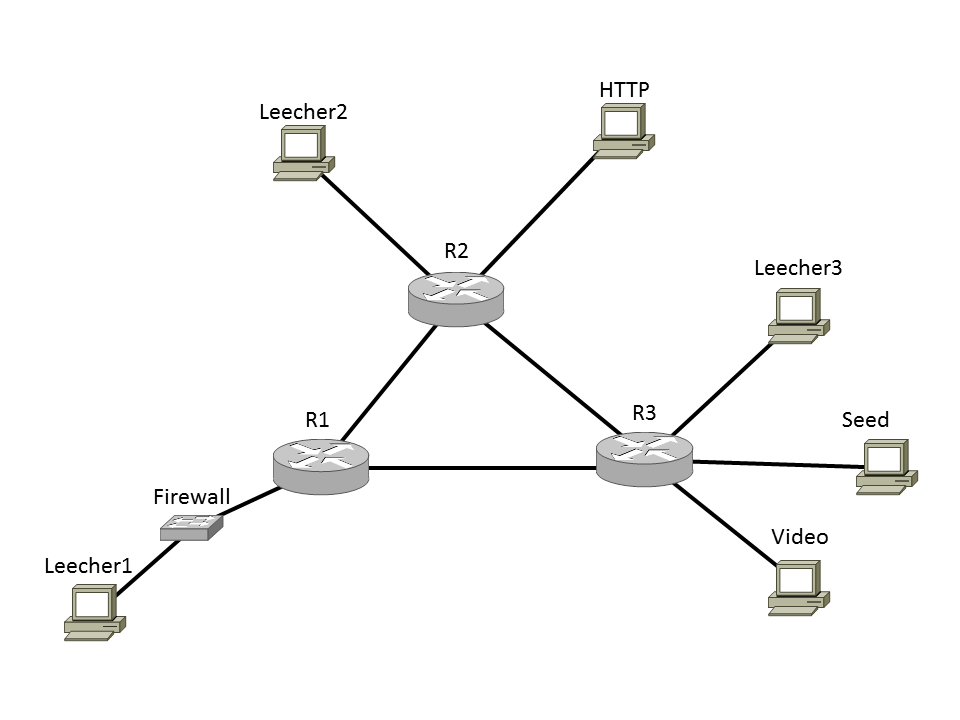
\includegraphics[width=0.9\textwidth]{figures/halozat.png}
    \caption{Network architecture used in lab exercises}
    \label{fig:Lab-topo}
\end{figure}

A hálózatban 4 OpenFlow switch fut, ezekböl 3 (R1, R2, R3) router müködést szimulál static routeokkal. Kiemelendö a
szimuláció, ugyanis az OpenFlow switchek nem képesek ARP kérésekre válaszolni, így azokat vagy egy megfelelö kontroller
alkalmazásból kell kezelni, vagy esetünkben static MAC címeket használunk. A szimulált hálózatban alapszabály, hogy a
hostok a saját routereiket mint gatewayt mindig a csupa nullás (egyébként invalid) MAC címmel érhetik el. A hostok MAC
címjei pedig "00:00:<ROUTER-ID>:00:00:<ROUTER-LINK-ID>" séma alapján kerül kiosztásra. Ennek megfelelöen az R2-es
routerre kötött elsö host (leecher 2) a "00:00:02:00:00:01" MAC címmel rendelkezik.

Az R2-es routeren a következö OpenFlow statikus szabályok kerülnek beillesztésre:

\begin{lstlisting}[language=bash,frame=single,breaklines,caption={R2 router flow entry configuration},label=lst:R2-flow-config]
ovs-ofctl add-flow r2 'ip,nw_dst=89.97.0.0/16,action=mod_dl_src:00:00:00:00:00:00,output:4'
ovs-ofctl add-flow r2 'ip,nw_dst=201.42.54.65/28,action=mod_dl_src:00:00:00:00:00:00,output:5'
ovs-ofctl add-flow r2 'ip,nw_dst=23.53.32.53/32,action=mod_dl_dst:00:00:02:00:00:01,output:1'
ovs-ofctl add-flow r2 'ip,nw_dst=23.99.30.4/32,action=mod_dl_dst:00:00:02:00:00:02,output:2'
ovs-ofctl add-flow r2 'ip,nw_dst=23.0.3.78/32,action=mod_dl_dst:00:00:02:00:00:03,output:3'
ovs-ofctl add-flow r2 'arp,action=output:1,2,3' 
\end{lstlisting}

Az elsö két szabály a két szomszédos router IP cím tartományát fedi le. Látható, hogy a szomszédos routerek tartományai
/16 és /28-as netmaskkal rendelkeznek. Ha ezekben az IP tartományokban érkezik egy csomag, akkor történik egy forrás
MAC állítás (cél MAC állításra is szükség lenne a pontos router müködés szimulálására, de esetünkben ez kihagyható,
mivel a túloldalon is általunk programozott OpenFlow eszköz van - egyszerübb flow bejegyzések) és kiküldés a megfelelö
porton. Hostok esetében a match pontosan akkor törénik, ha az IP címnek mind a 32 bitje felveszi a célcímben megadott
IP címet. Egyezés esetén a cél MAC a host MAC címe lesz, és kiküldi a switch/router a megfelelö porton. Az utolsó sor
azt a könnyítést adja, hogy ugyanazon a subneten levö hostoknak (azaz ugyanarra a switchre/routerre bekötött) ne
kelljen statikusan megadni a MAC címjeit. Mivel az ARP egy broadcast címre épülö protokoll, ezért floodolni kell,
ugyanakkor figyelemben kell tartani, hogy nem minden portra kell floodolni. A router szétbontja a hálózatokat broadcast
domainekre, így a router szimulációjánál is figyelembe kell venni ezt a tulajdonságot. Ha az OpenFlow switchnek flood
paramétert adnánk meg, akkor a többi routert szimuláló switchnek is elküldenénk, amik szintúgy továbbítanák minden
portjukon, azaz egyetlen ARP csomag képes olyan broadcast stormot generálni, ami megbénítja a Mininet szimulációt
futtató gazdagépet.

A 4. switch (Firewall) nem rendelkezik statikus OF bejegyzésekkel, tisztán a kontrollertöl függ. A mérési feladatok
során a kontroller programozásával kell szürésí intelligenciát vinni a tüzfalba, hogy a torrent forgalmat megfelelöen
szürje, vagy éppen shape-elje. A tüzfal két porttal rendelkezik, és alapbeállításban a kontroller egy repeater funkciót
valósít meg a switchen, azaz ami egyik porton beérkezik, az a másikon kimegy. A tüzfal a kontroller fele Packet-In
üzenetekben küldi az egyik porton beérkezett csomagot, és ennek megfelelöen a POX kontroller alkalmazás a
handlePacketIn metódusában kezeli le ezeket a csomagokat. Az intelligenciát is ebben a metódusban kell implementálni. A
beérkezett csomag parsolását a következö függvényhívás végzi:
\begin{lstlisting}[language=python,frame=single,breaklines]
packet = event.parsed  
\end{lstlisting}

Ez után a 'packet' objektumtól már egyszerüen lekérdezhetöek az OpenFlow által ismert paraméterek. Például a beérkezö
port sorszáma a "packet.port", míg egy specifikus TCP port megtalálása és szürése a következöképpen nézhet ki:

\begin{lstlisting}[language=python,frame=single,breaklines]
tcpp = event.parsed.find( 'tcp' )

if not tcpp: return # Not TCP

if tcpp.srcport in block_ports or tcpp.dstport in block_ports:

# Halt the event, stopping l2_learning from seeing it

# (and installing a table entry for it)

core.getLogger( "blocker" ).debug( "Blocked TCP %s <-> %s" ,

tcpp.srcport, tcpp.dstport)

event.halt = True
\end{lstlisting}

Mivel az OpenFlow nem néz L4-nél magasabb rétegekbe, ezért például egy BitTorrent csomag header mezöinek az elemzése
problémásabb, ilyenkor muszáj az L4-es payload elemzése a "payload" property segítségével.

\appendix

\section{Entry quiz sample questions}

\section{Input files for the lab excercise}
\begin{itemize}

    \item

          \href{https://qosip.tmit.bme.hu/foswiki/pub/Meres/P2PAlkalmazasokMeresiSegedlet/p2pMeresTopo.py.txt}{p2pMeresTopo.py.tx
              t}: Mininet topologia P2P mereshez, futtatas: 'sudo python p2pMeresTopo.py'

    \item

          \href{https://qosip.tmit.bme.hu/foswiki/pub/Meres/P2PAlkalmazasokMeresiSegedlet/p2pMeresTopo.py.txt}{p2p.py.txt}: POX
          kontroller alkalmazas, bemasolando pox/ext konyvtarba, futtatas: './pox.py p2p'
\end{itemize}

\section{Lab exercises}

\end{document}